\documentclass[11pt]{beamer}
\usetheme{Dresden}
%\usecolortheme{beaver}
\usepackage[utf8]{inputenc}
\usepackage{amsmath}
\usepackage{amsfonts}
\usepackage{amssymb}
\usepackage{graphicx}
\usepackage{verbatim}
\usepackage{listings}
\usepackage{xcolor}

  \setbeamertemplate{footline}%{miniframes theme}
  {%
    \begin{beamercolorbox}[colsep=1.5pt]{upper separation line foot}
    \end{beamercolorbox}
    \begin{beamercolorbox}[ht=2.5ex,dp=1.125ex,%
      leftskip=.3cm,rightskip=.3cm plus1fil]{author in head/foot}%
      \leavevmode{\usebeamerfont{author in head/foot}\insertshortauthor}%
      \hfill%
      {\usebeamerfont{institute in head/foot}\usebeamercolor[fg]{institute in head/foot}\insertshortinstitute}%
    \end{beamercolorbox}%
    \begin{beamercolorbox}[ht=2.5ex,dp=1.125ex,%
      leftskip=.3cm,rightskip=.3cm plus1fil]{title in head/foot}%
      {\usebeamerfont{title in head/foot}\insertshorttitle} \hfill     \insertframenumber%
    \end{beamercolorbox}%
    \begin{beamercolorbox}[colsep=1.5pt]{lower separation line foot}
    \end{beamercolorbox}
  }

\let\OldTexttt\texttt
\renewcommand{\texttt}[1]{\OldTexttt{\color{teal}{#1}}}

\definecolor{mGreen}{rgb}{0,0.6,0}
\definecolor{mGray}{rgb}{0.5,0.5,0.5}
\definecolor{mPurple}{rgb}{0.58,0,0.05}
\definecolor{mGreen2}{rgb}{0.05,0.65,0.05}
\definecolor{mGray2}{rgb}{0.55,0.55,0.55}
\definecolor{mPurple2}{rgb}{0.63,0.05,0.05}
\definecolor{backgroundColour}{rgb}{0.95,0.95,0.92}
\definecolor{backgroundColour2}{rgb}{0.95,0.92,0.95}

\lstdefinestyle{C}{
    backgroundcolor=\color{backgroundColour},   
    commentstyle=\color{mGreen},
    keywordstyle=\color{blue},
    numberstyle=\tiny\color{mGray},
    stringstyle=\color{mPurple},    
    basicstyle=\footnotesize,
    breakatwhitespace=false,         
    breaklines=true,                 
    captionpos=b,                    
    keepspaces=true,                 
    numbers=left,                    
    numbersep=5pt,                  
    showspaces=false,                
    showstringspaces=false,
    showtabs=false,                  
    tabsize=2,
    language=C
}

\lstdefinestyle{Python}{
    backgroundcolor=\color{backgroundColour2},   
    commentstyle=\color{mGreen2},
    keywordstyle=\color{blue},
    numberstyle=\tiny\color{mGray2},
    stringstyle=\color{mPurple2},
    basicstyle=\footnotesize,
    breakatwhitespace=false,         
    breaklines=true,                 
    captionpos=b,                    
    keepspaces=true,                 
    numbers=left,                    
    numbersep=5pt,                  
    showspaces=false,                
    showstringspaces=false,
    showtabs=false,                  
    tabsize=2,
    language=Python
}

\definecolor{eggplant}{rgb}{0.5, 0.25, 0.5} % UBC Blue (primary)

\usecolortheme[named=eggplant]{structure}

\author{NCC Moore}
\title{Topic 8 - Pointers in C}
%\setbeamercovered{transparent} 
%\setbeamertemplate{navigation symbols}{} 
%\logo{} 
\institute{McMaster University} 
\date{Fall 2020} 
\subject{COMPSCI 1XC3 - Computer Science Practice and Experience: Development Basics} 
\stepcounter{section}
\begin{document}

\begin{frame}
\center
COMPSCI 1XC3 - Computer Science Practice and Experience:
Development Basics
\titlepage
% Toggle for C chapters
Adapted from C: How to Program 8th ed., Deitel \& Deitel
\end{frame}

\begin{frame}
\tableofcontents
\end{frame}

\section[Syntax]{Working with Pointers} % include 
\begin{frame}{Pointers in C}
\center
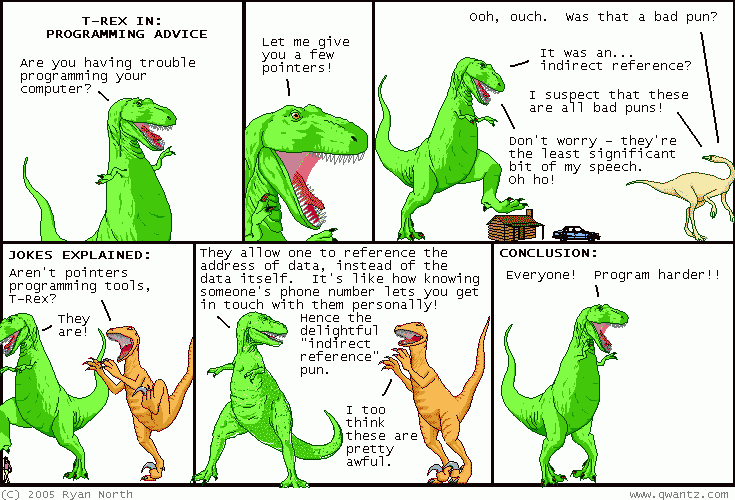
\includegraphics[scale=0.28]{DCPointers.png} \\
"When a wise man points at the moon \\the imbecile examines the finger" \\
-- A person a lot of quotes get attributed to -- 
\end{frame}

\begin{frame}{So what the heck's a pointer and why should I care?}
Pointers are one of the most \textit{powerful} constructs in C.
\begin{itemize}
\item A \textbf{pointer} is a variable whose value is a \textbf{memory address}.
\item Where most variables directly reference the value stored at some position in memory, pointers are \textbf{indirect references}.  
\item In this set of slides we're going to talk about:
\begin{itemize}
\item Pointer Data Types
\item Pointer Operations
\item Applications of Pointers
\end{itemize}
\end{itemize}
\end{frame}

\begin{frame}[fragile=singleslide]{Pointerization!}
A pointer is not declared as a new datatype, but as a modifier to existing data types.
\begin{lstlisting}[style = C]
int* ptr;
\end{lstlisting}
The \texttt{*} character indicates that \texttt{ptr} is an \textbf{integer pointer}.  
\begin{itemize}
\item This is to say, \texttt{ptr} points to a segment of memory the size of an \texttt{int}.  
\end{itemize}
The \texttt{*} character may be applied to either the data type or the identifier itself:
\begin{lstlisting}[style = C]
int *countPtr, count;
\end{lstlisting}
\begin{itemize}
\item \texttt{*} only pointerizes \texttt{countPtr} in this example.  
\item If \texttt{*} were applied to \texttt{int}, \texttt{countPtr} would still be the only variable that was pointerized.
\end{itemize}
\end{frame}

\begin{frame}{In Blue Block-o-vision...}
\center
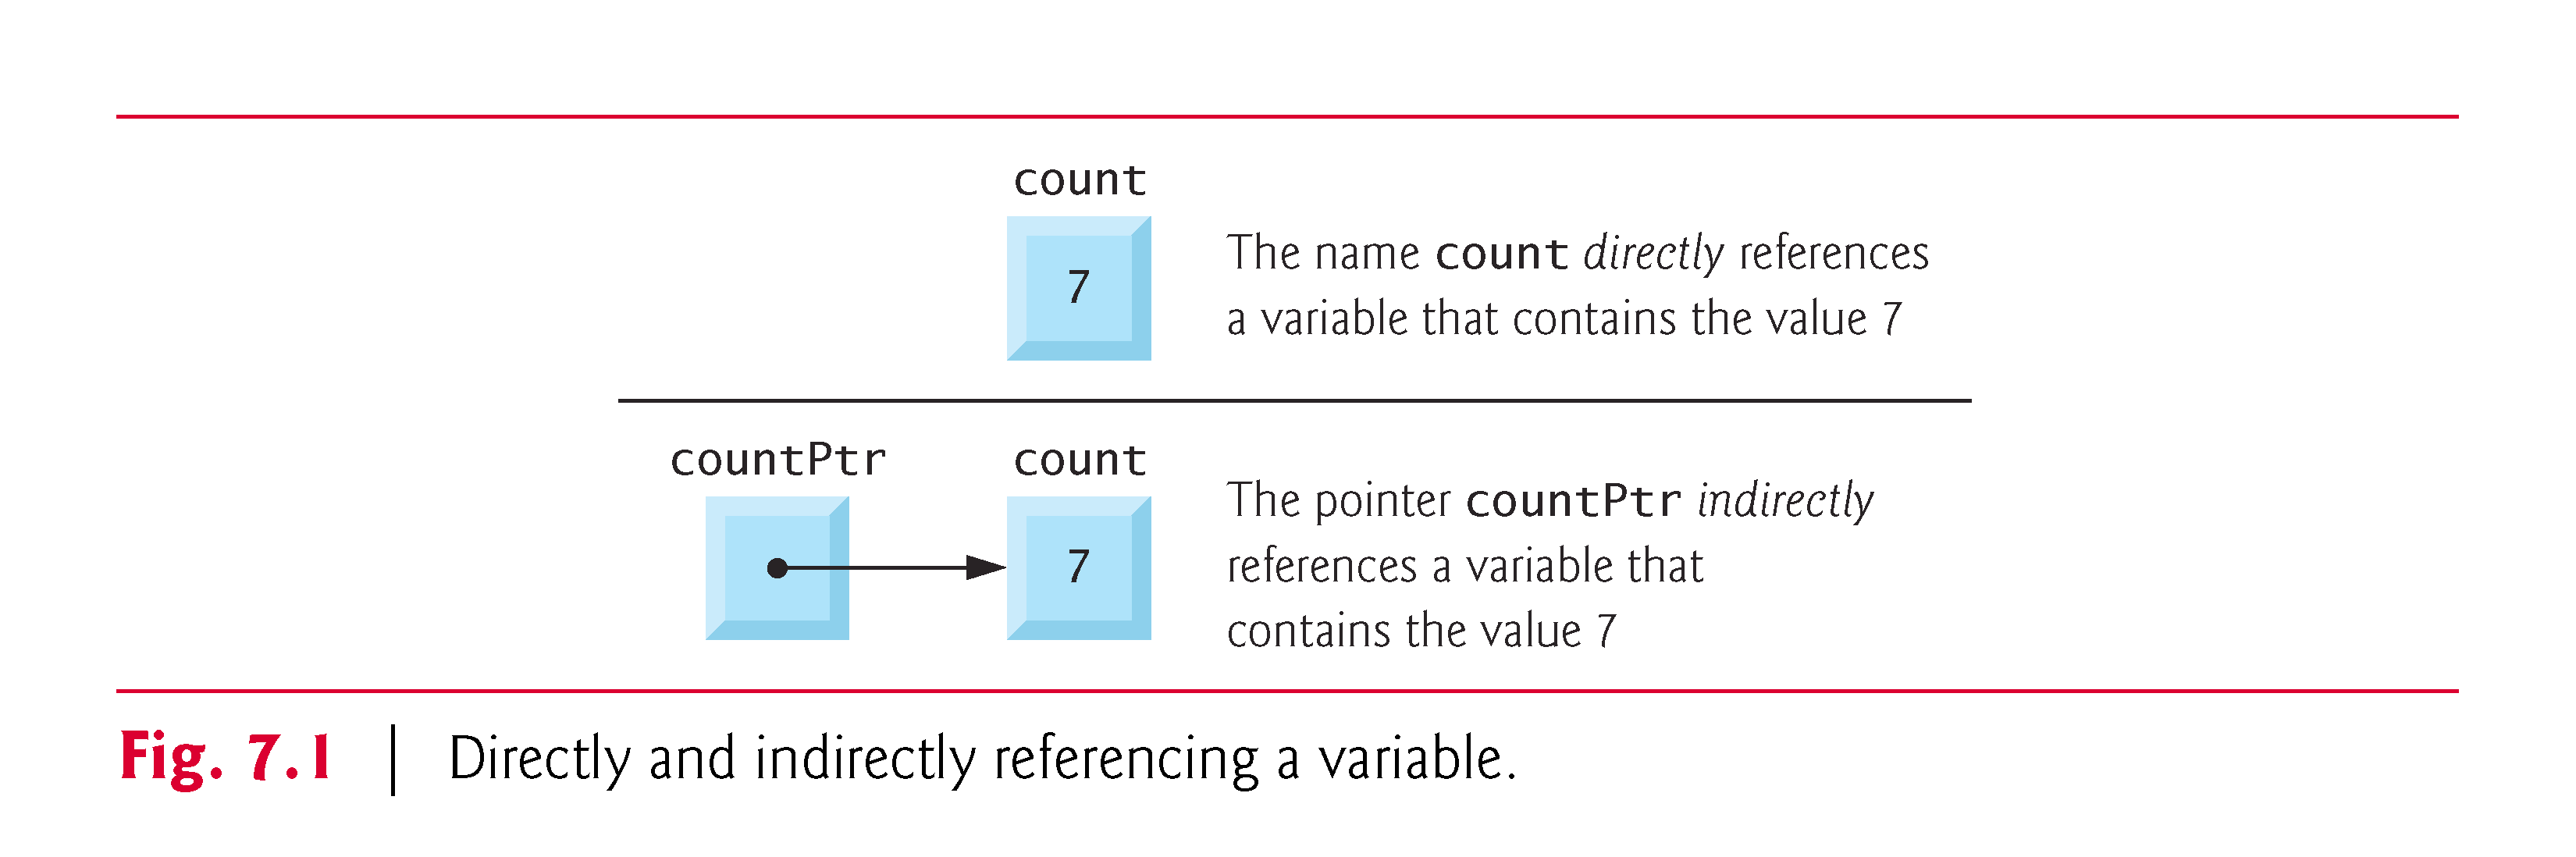
\includegraphics[scale=0.125]{tba.png}
\end{frame}

\begin{frame}{Pointer Facts}
\begin{itemize}
\item You can create a pointer out of \emph{any} datatype, including custom ones.
\item \texttt{*} means something different when you're not declaring a pointer... \emph{it's not part of the identifier!}
\item Since pointers are a more direct manipulation of memory, you can squeeze out some efficiencies by squeezing in some pointers! 
\end{itemize}
Stylistic Points
\begin{itemize}
\item To avoid the confusion on the previous slide, it's better to declare pointers and direct variables on separate lines.
\item Putting some indication that a variable is a pointer in the identifier is a good way to be able to tell which variables are pointers later on.  
\end{itemize}
\end{frame}

\begin{frame}[fragile=singleslide]{Initial Pointing}
Like a lot of things in C, uninitialized pointers contain junk data.  
\begin{itemize}
\item A pointer will initially point to a random memory cell! 
\item Pointers should be initialized to either 0, \texttt{NULL} or a value that makes sense.
\begin{itemize}
\item \texttt{NULL} is a \textbf{symbolic constant}, which is defined in a number of header files (such as \texttt{stdio.h} and \texttt{ stddef.h})
\item \texttt{NULL} is the same thing as zero, but it's preferred for stylistic reasons.
\end{itemize}
\end{itemize}
\begin{lstlisting}[style = C]
int* ptr = NULL;
if (ptr != NULL) {
	// do stuff
}
\end{lstlisting}
\end{frame}

\section[Operations]{Pointer Operations!}
\begin{frame}[fragile=singleslide]{We've done the nouns, here come the verbs...}
Now we know how to store a memory address, but what good is it if we have no addresses to store?
\begin{itemize}
\item Memory Adresses are accessed using \texttt{\&}, the ``address of'' operator.
\item Applied to any identifier, it returns the physical memory address of that identifier. 
\item This includes pointers! 
\end{itemize}
\begin{lstlisting}[style = C]
int y = 5;
int* yPtr;
// store the address of y in yPtr
yPtr = &y;
\end{lstlisting}
\end{frame}

\begin{frame}{Address of Operator in Box-O-Vision}
\center
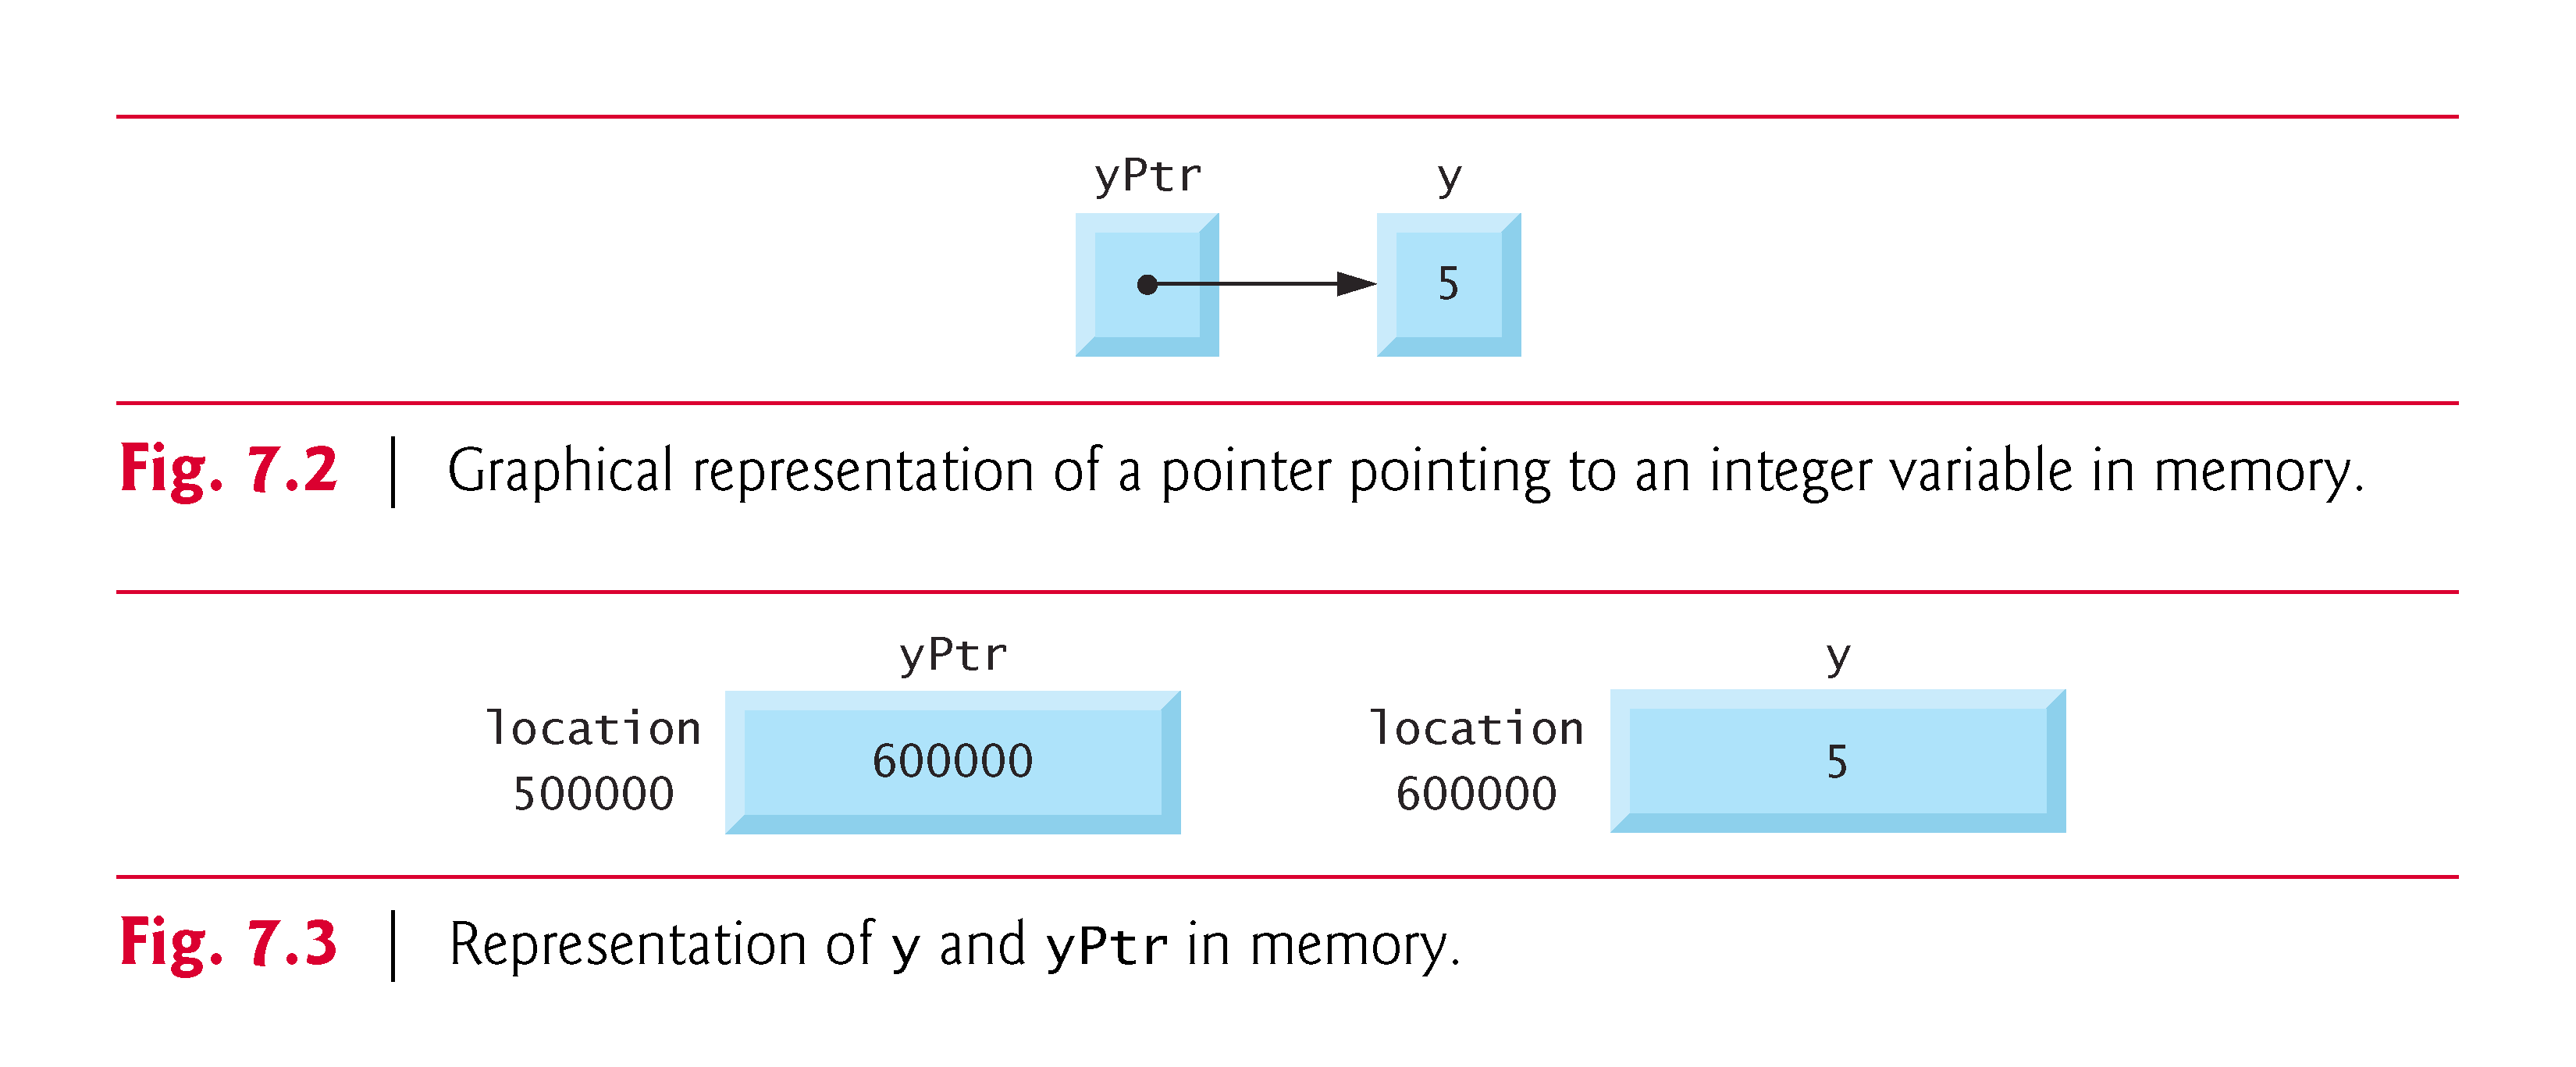
\includegraphics[scale=0.12]{tbb.png}
\end{frame}

\begin{frame}[fragile=singleslide]{Dereferencing for Fun and Profit}
The inverse operation of \texttt{\&} is \textbf{pointer dereferencing}
\begin{itemize}
\item This is a little confusing, but it's also \texttt{*}.
\item Additionally, the formatter for pointers is \texttt{\%p}.
\end{itemize}
\begin{lstlisting}[style = C]
int y = 5;
int* yPtr;
// store the address of y in yPtr
yPtr = &y;
printf("The pointer's value is %p\n", yPtr);
printf("The value pointed to is %d", *yPtr);
\end{lstlisting}
\hrule
\begin{verbatim}
The pointer's value is 0x7ffe0fba22fc
The value pointed to is 5
\end{verbatim}
\end{frame}

\begin{frame}{The Deadly and Dreaded SEGFAULT}
Dereferencing a pointer that points to memory outside your program's allocated memory space causes a fatal runtime error called a \textbf{segmentation fault}.
\center
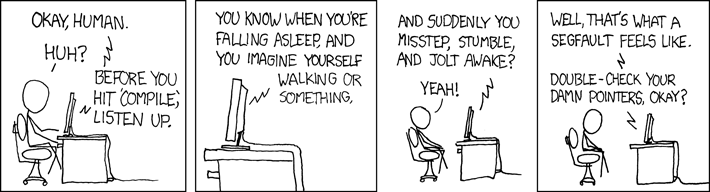
\includegraphics[scale=0.4]{compiler_complaint.png}
This is most common with \texttt{NULL} pointers, but can also happen if you mess up your pointer arithmetic.
\end{frame}

\begin{frame}[fragile=singleslide]{\texttt{\&} and \texttt{*} are Inverse Operations}
\begin{lstlisting}[style=C]
#include <stdio.h>
int main(void) {
	int a = 7;
	int *aPtr = &a;
	printf("a = %d\n", a);
	printf("&a = %p\n", &a);
	printf("aPtr = %p\n", aPtr);
	printf("*aPtr = %d\n", *aPtr);
	printf("Generating a memory address and dereferencing it\nleaves you where you started.\n");
	printf("*&a = %d\n", *&a);
	printf("The other way around causes an actual compiler error...\n");
//	printf("&*a = %d", &*a);
}
\end{lstlisting}
\end{frame}

\begin{frame}[fragile=singleslide]{\texttt{\&} and \texttt{*} are Inverse Operations (Output)}
\begin{verbatim}
a = 7
&a = 0x7ffe08ed2edc
aPtr = 0x7ffe08ed2edc
*aPtr = 7
Generating a memory address and then dereferencing it
leaves you where you started.
*&a = 7
The other way around causes an actual compiler error...
\end{verbatim}
\end{frame}

\begin{frame}[fragile=singleslide]{Arrays of Pointers!}
It can be easy to think of pointers entirely symbolically, and forget that they too have concrete values in memory.
\begin{itemize}
\item Pointers may be collected and organized in arrays, just like other data types.  
\end{itemize}
\begin{lstlisting}[style=C]
const char *suit[4] 
    = {"Hearts", "Diamonds", "Clubs", "Spades"};
\end{lstlisting}
\begin{itemize}
\item Each element in the array is a pointer to a character array.
\item The fact that our array contains pointers, instead of the character arrays themselves, means the character arrays' memory is managed separately from the array of pointers.
\item Whereas a 2D array must be rectangular, each character array pointed to by the array of pointers may have a unique length! 
\end{itemize}
\end{frame}

\begin{frame}{Arrays of Pointers in Block-O-Vision}
\center
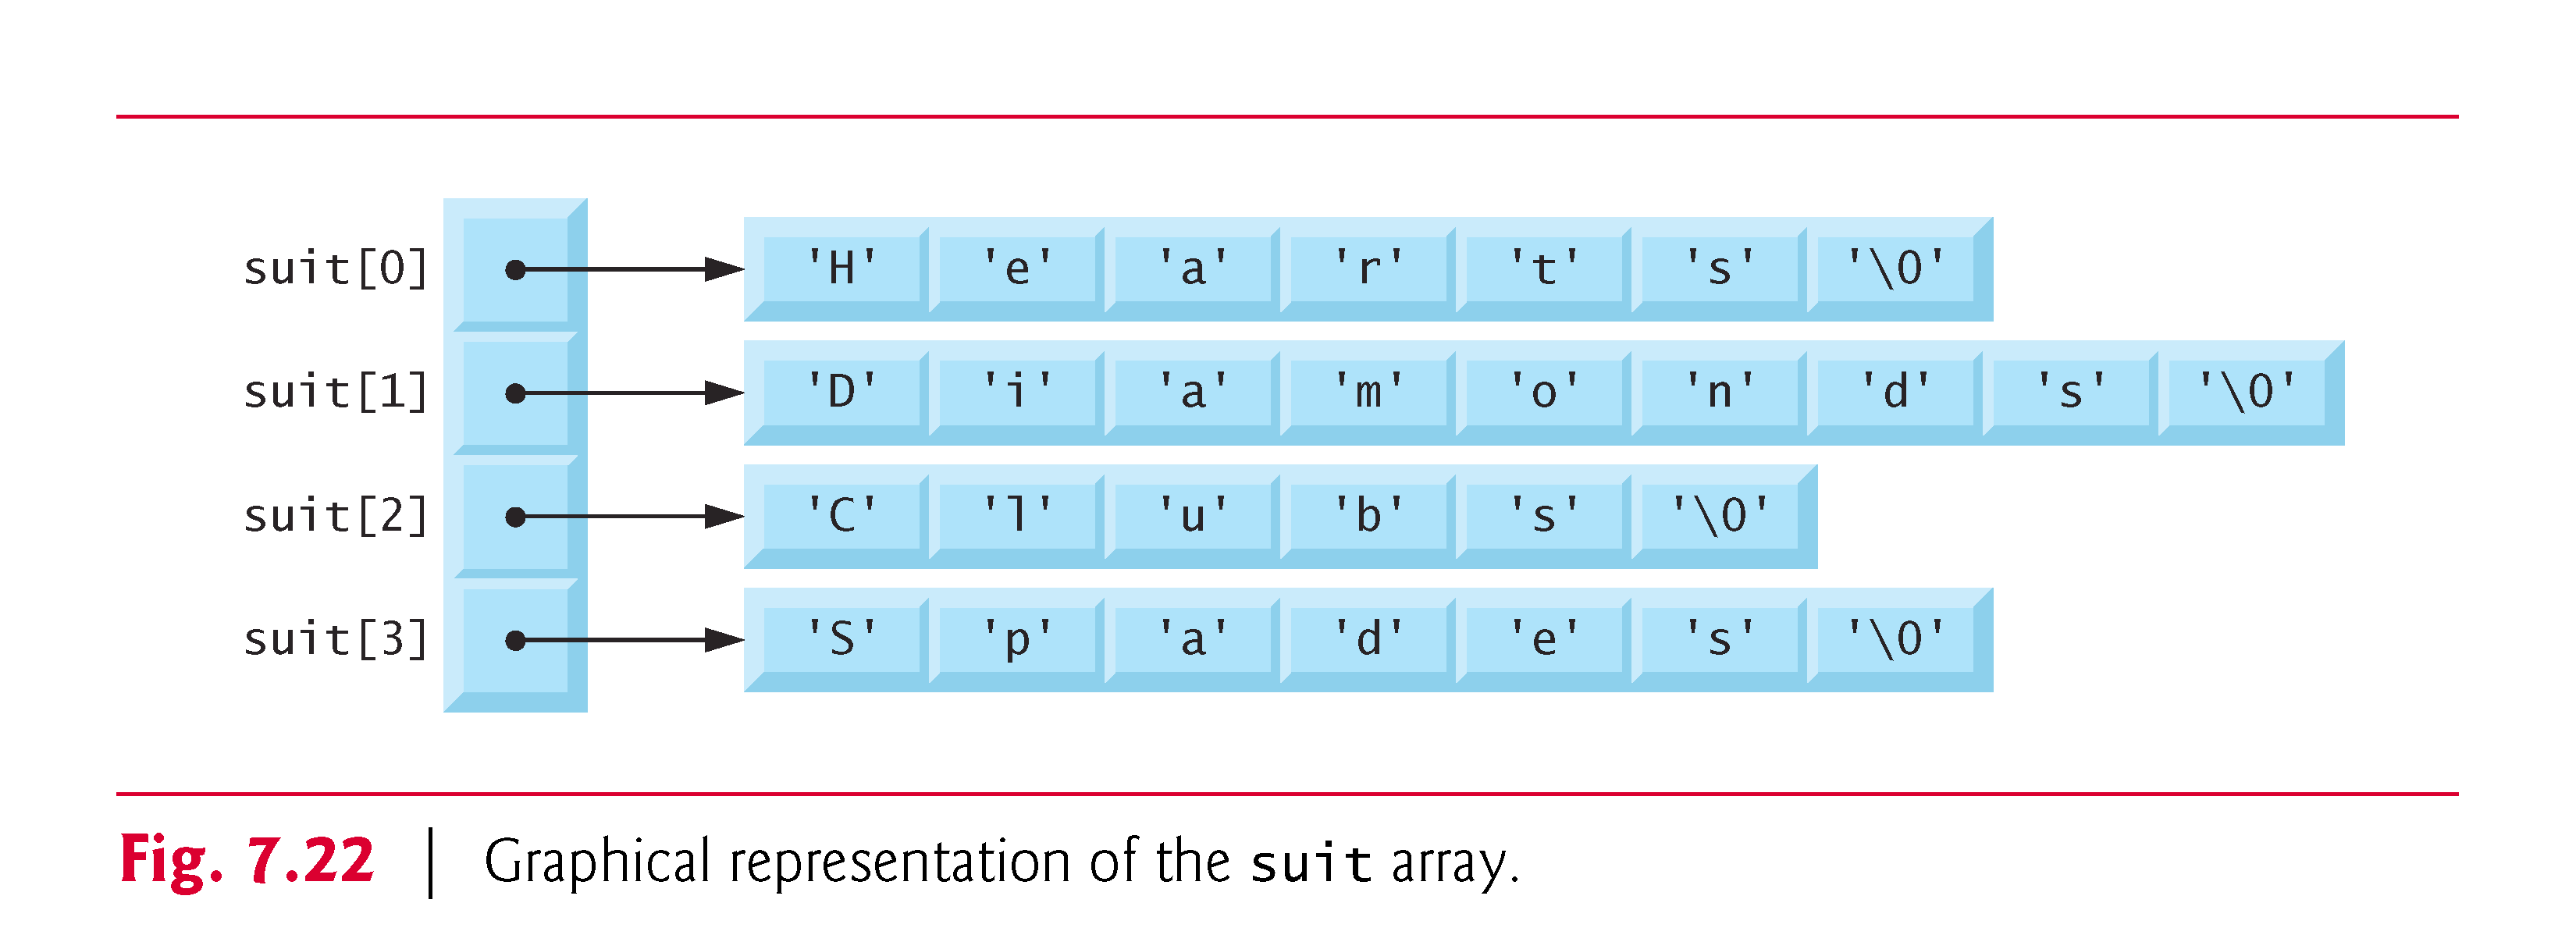
\includegraphics[scale=0.1]{tbf.png}
\end{frame}

\section[Passing]{The Wonderful World of Passing by Reference}
\begin{frame}[fragile=singleslide]{Proud and Practical Pointer Passing}
\begin{itemize}
\item All arguments are passed by value by C... Unless the value you pass is a memory address!
\item Passing by reference allows functions to modify the referred data in the calling function, which can be useful!
\begin{lstlisting}[style=C]
int foo;
int bar[];
myFunc(&foo, bar);
\end{lstlisting}
\item We use \texttt{\&} to pass the address of \texttt{foo}, but \texttt{bar} is already a memory address.
\item In C, \texttt{someArray} $\equiv$ \texttt{\&someArray[0]}.
\item Inside the function definition, \texttt{foo} will need to be dereferenced, but \texttt{bar} will not.
\end{itemize}
\end{frame}

\begin{frame}[fragile=singleslide]{Example: Cube By Reference}
\begin{lstlisting}[style=C]
#include <stdio.h>

void cubeByReference(int *nPtr);

int main(void) {
	int num = 5;
	printf("num = %d\n", num);
	cubeByReference(&num);
	printf("num = %d\n", num);
}

void cubeByReference(int *nPtr){
	*nPtr = *nPtr * *nPtr * *nPtr;
}
\end{lstlisting}
\end{frame}

\begin{frame}{In Block-O-Vision...}
\center
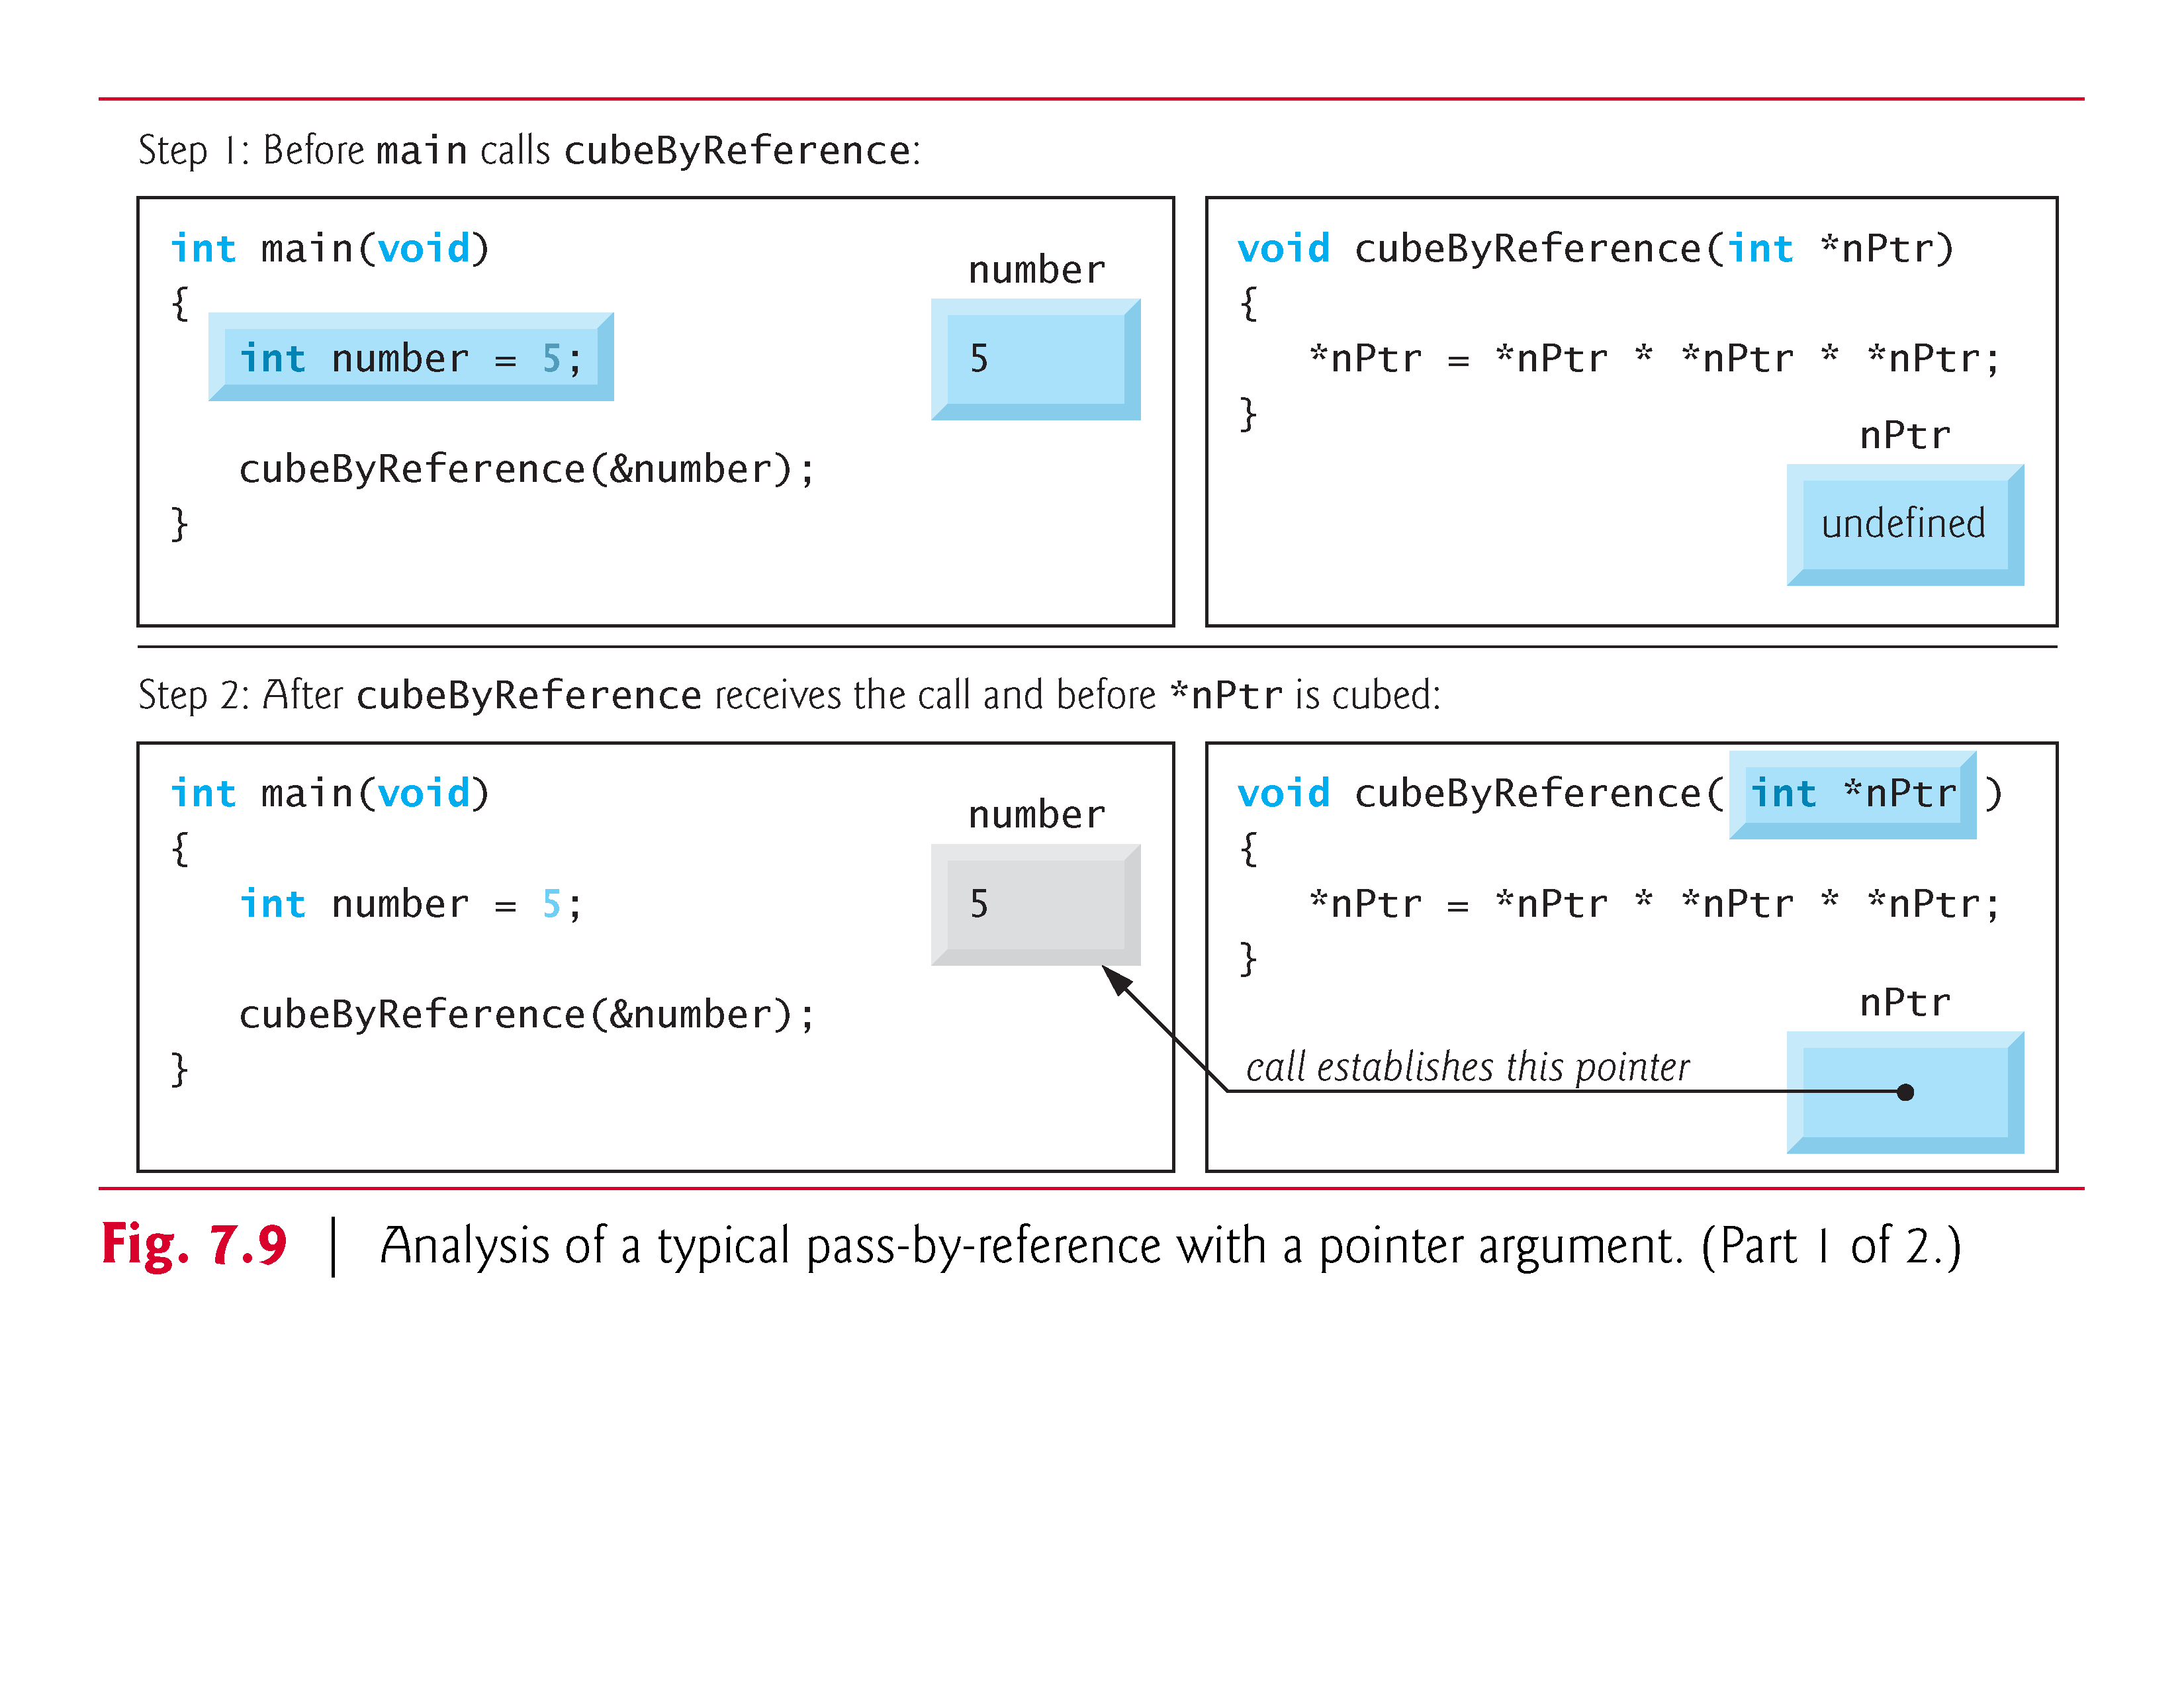
\includegraphics[scale=0.35]{tbc.png}
\end{frame}

\begin{frame}{In Block-O-Vision...}
\center
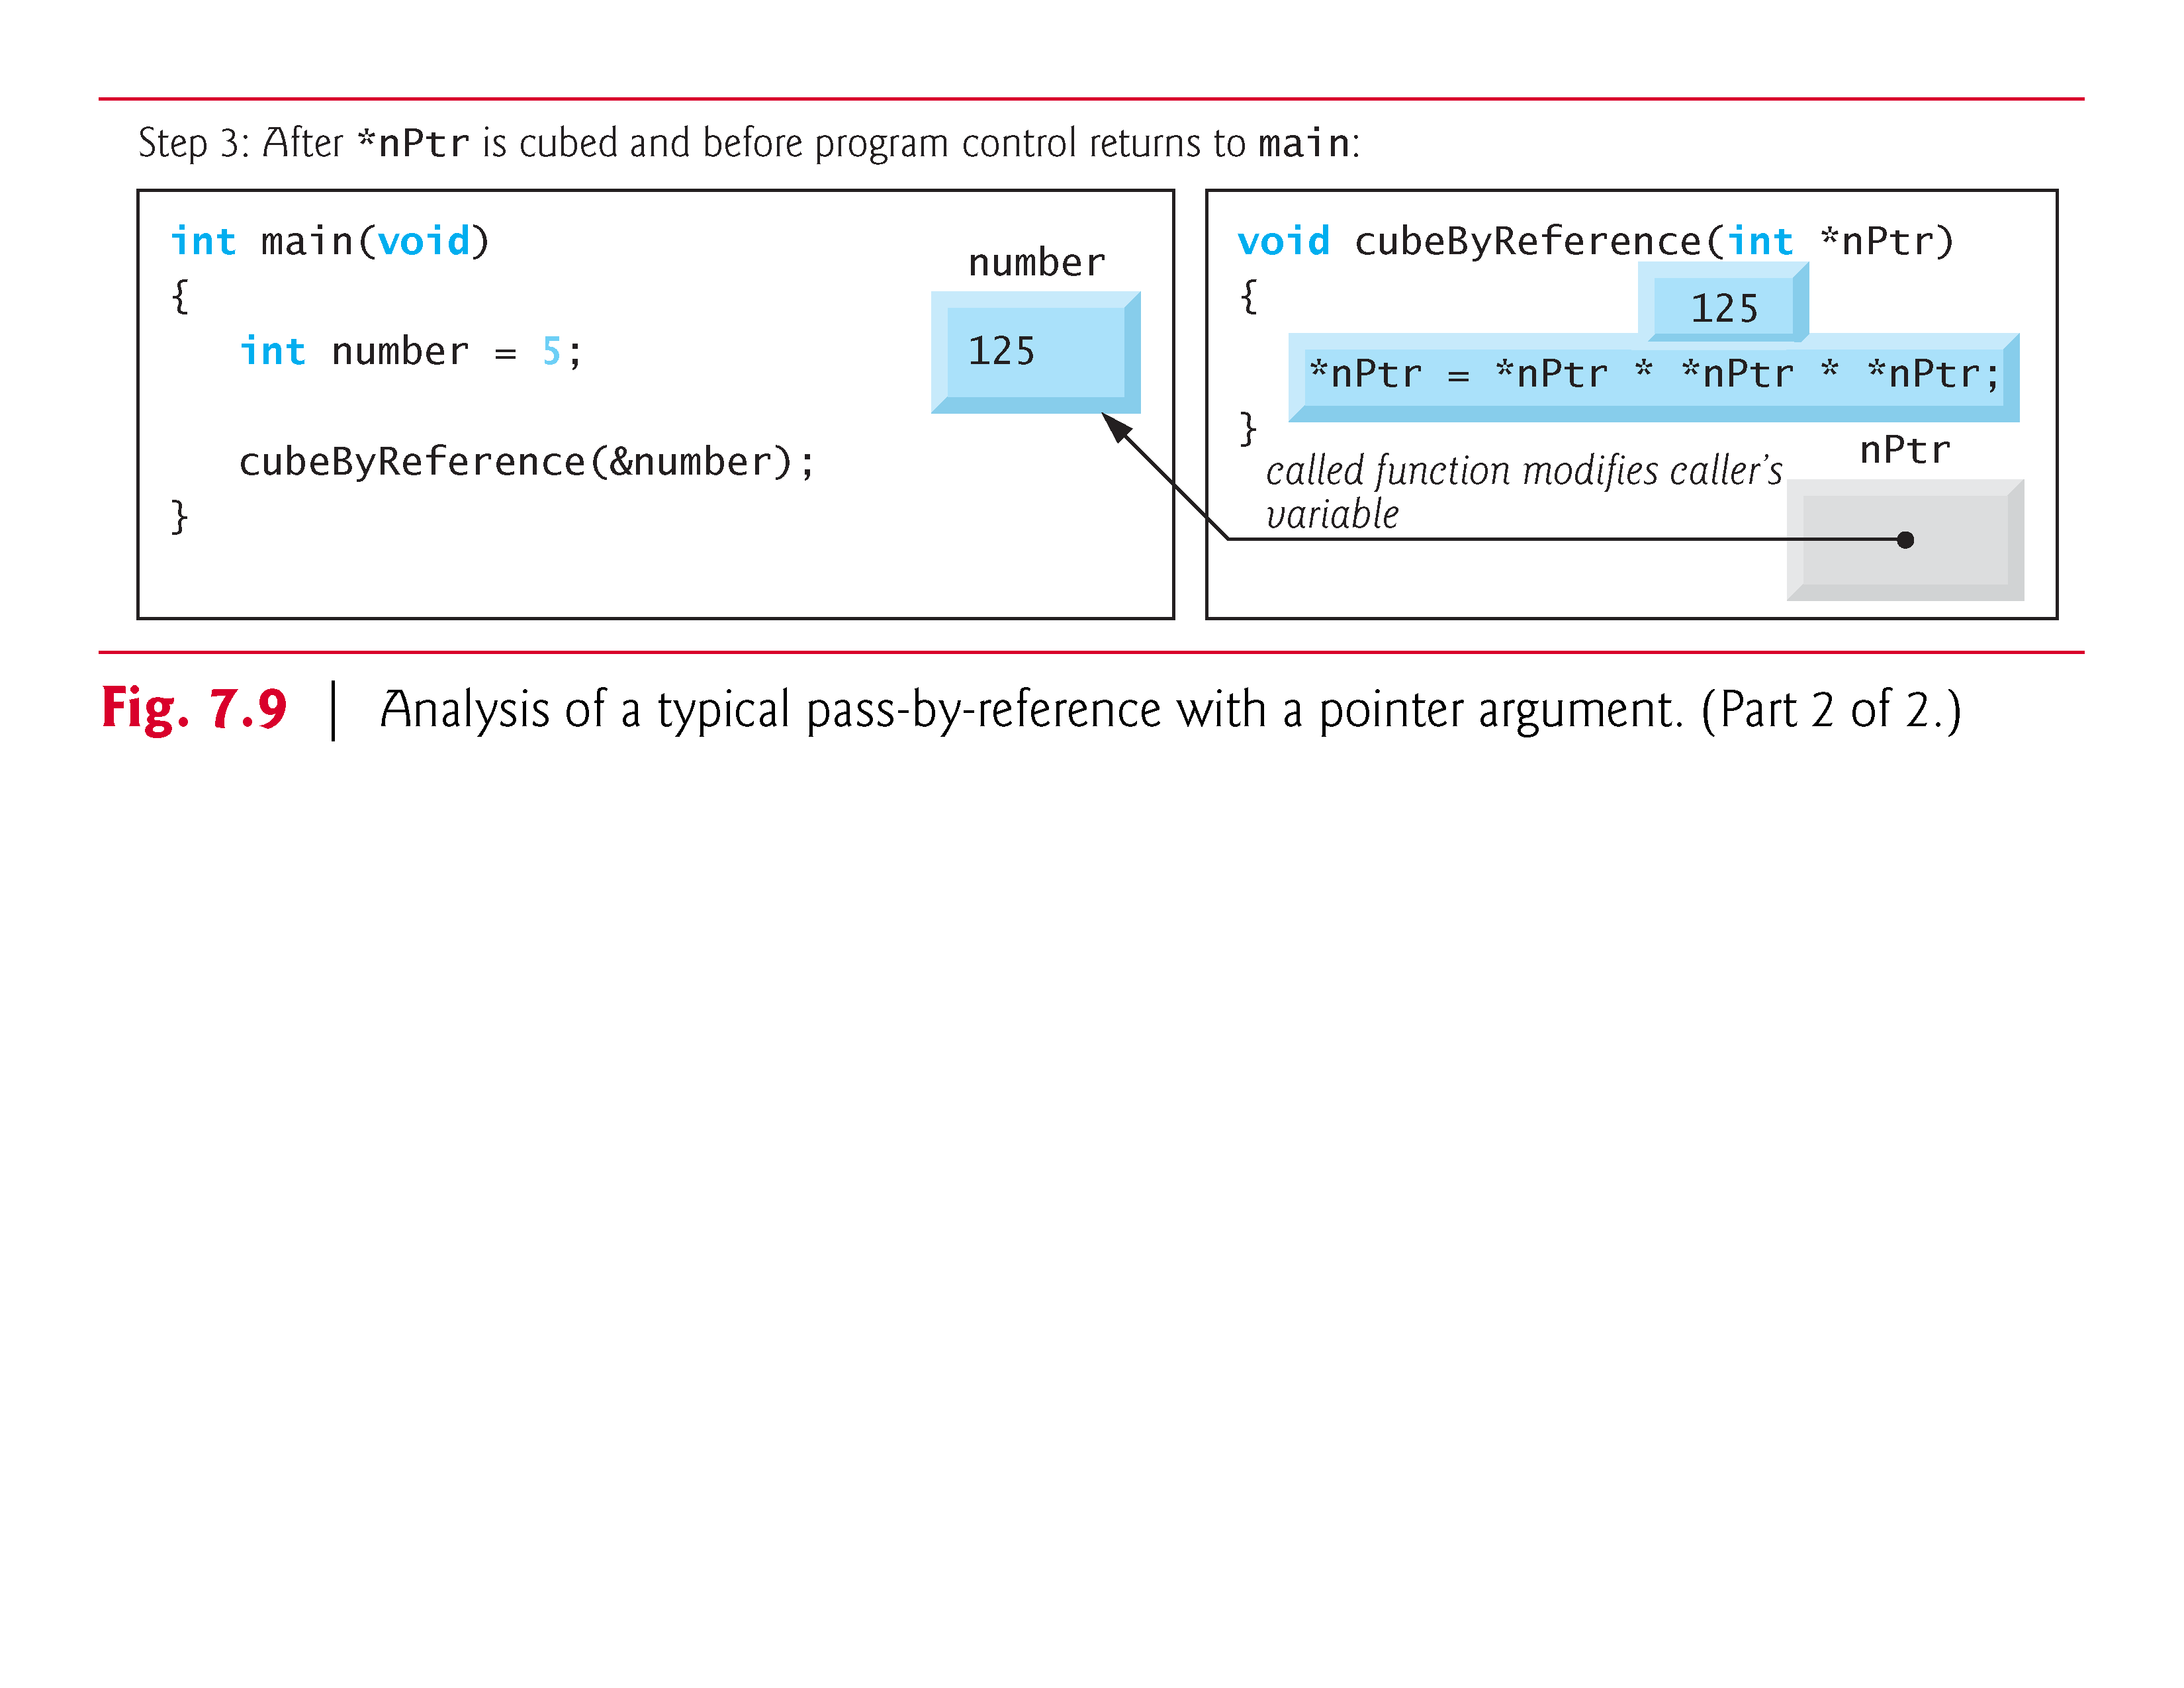
\includegraphics[scale=0.35]{tbd.png}
\end{frame}

\begin{frame}[fragile=singleslide]{Example: Cube By Reference}
\begin{itemize}
\item In order to accept a memory address as an argument, the fact must be specified in the argument's type information.
\item In this example, we replace the following operations: 
\begin{itemize}
\item Pass \texttt{num} by value to \texttt{cubeByReference}
\item Compute the cube and return it to \texttt{main}
\item Assign the return value of \texttt{cubeByReference} to \texttt{num}
\end{itemize}
\item With this:
\begin{itemize}
\item Pass the address of \texttt{num} to \texttt{cubeByReference}
\item Compute the cube and store it in the memory address directly
\end{itemize}
\item Stylistically, pass by value is preferred unless the situation explicitly calls for pass by reference.
\begin{itemize}
\item Passing by reference in this way violates the \textbf{principle of least privilege}.
\end{itemize}
\end{itemize}
\end{frame}

\begin{frame}{Arrays Are Pointers!}
The syntax for passing an array as an argument to a function is the same as passing a variable by reference.  
\begin{itemize}
\item This is because the compiler does not differentiate between pointers and one-dimensional arrays.  
\begin{itemize}
\item Like so many things in C, that means it's your job! 
\item It's up to you to write your functions so that they are using their arguments as intended!  
\item Documentation becomes critical!
\end{itemize}
\item An array is actually a pointer to it's own first element.
\item We can perform arithmetic to traverse arrays without the indexing operator! 
\end{itemize}
\end{frame}

\begin{frame}[fragile=singleslide]{\texttt{const} and the Art of Mental Stillness}
Problem: Whenever we work with pointers, there's a possibility of pointer misuse resulting in a segfault! 
\begin{itemize}
\item We can prevent arguments from being modified by using the \texttt{const} qualifier.
\end{itemize}
\begin{lstlisting}[style=C]
void myFunc (const int *foo, float *bar);
\end{lstlisting}
\begin{itemize}
\item Trying to modify a \texttt{const} argument will result in the following compiler error using gcc:
\end{itemize}
\hrule
\begin{verbatim}
error: assignment of read-only location 
\end{verbatim}
\hrule
\begin{itemize}
\item Using \texttt{const} to restrict functions from modifying things they shouldn't modify is \emph{good software design!}
\item In general, a program should have only enough data access to accomplish it's task, and not one smidgeon more! 
\end{itemize}
\end{frame}

\section[Arith]{Pointer Expressions and Arithmetic}
\begin{frame}{Pointer Arithmetic}
\center
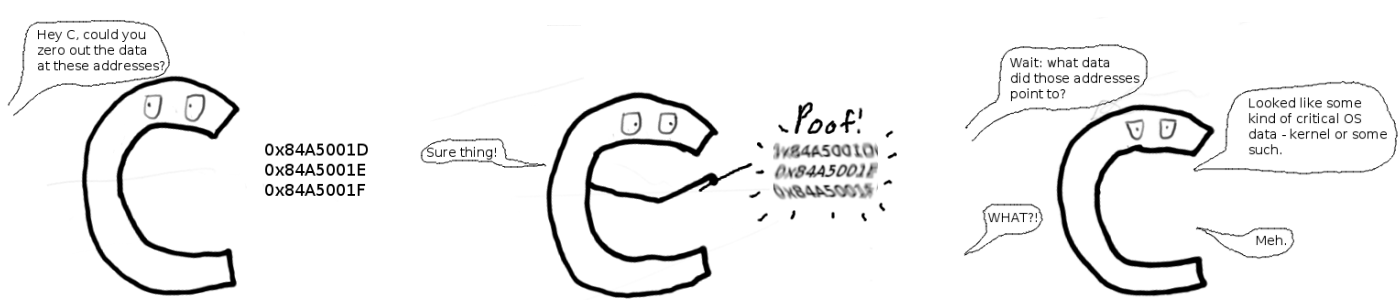
\includegraphics[scale=0.225]{c_os-files.png}
\\
\vspace{2em}
No clever quote this time, though I did learn the internet seems to think ``indirect'' means ``passive aggressive.''\\
-- The Prof -- \\
\end{frame}

\begin{frame}[fragile=singleslide]{A Program Illustrating Array Addressing}
\begin{lstlisting}[style=C]
#include<stdio.h>

int main(void){
	int foo[] = {0,1,2,3,4};
	short int bar[] = {0.0,1.0,2.0,3.0,4.0};
	printf("-----------------\n");
	for (int i = 0; i < 5; i++) {
		printf("&foo[%d] = %p\n", i, &foo[i]);
	}
	printf("-----------------\n");
	for (int i = 0; i < 5; i++) {
		printf("&bar[%d] = %p\n", i, &bar[i]);
	}
}
\end{lstlisting}
\end{frame}

\begin{frame}[fragile=singleslide]{Output of a Program Illustrating Array Addressing}
\begin{verbatim}
-----------------
&foo[0] = 0x7fff2f07b190
&foo[1] = 0x7fff2f07b194
&foo[2] = 0x7fff2f07b198
&foo[3] = 0x7fff2f07b19c
&foo[4] = 0x7fff2f07b1a0
-----------------
&bar[0] = 0x7fff2f07b186
&bar[1] = 0x7fff2f07b188
&bar[2] = 0x7fff2f07b18a
&bar[3] = 0x7fff2f07b18c
&bar[4] = 0x7fff2f07b18e
\end{verbatim}
\end{frame}

\begin{frame}{In Block-O-Vision}
\center
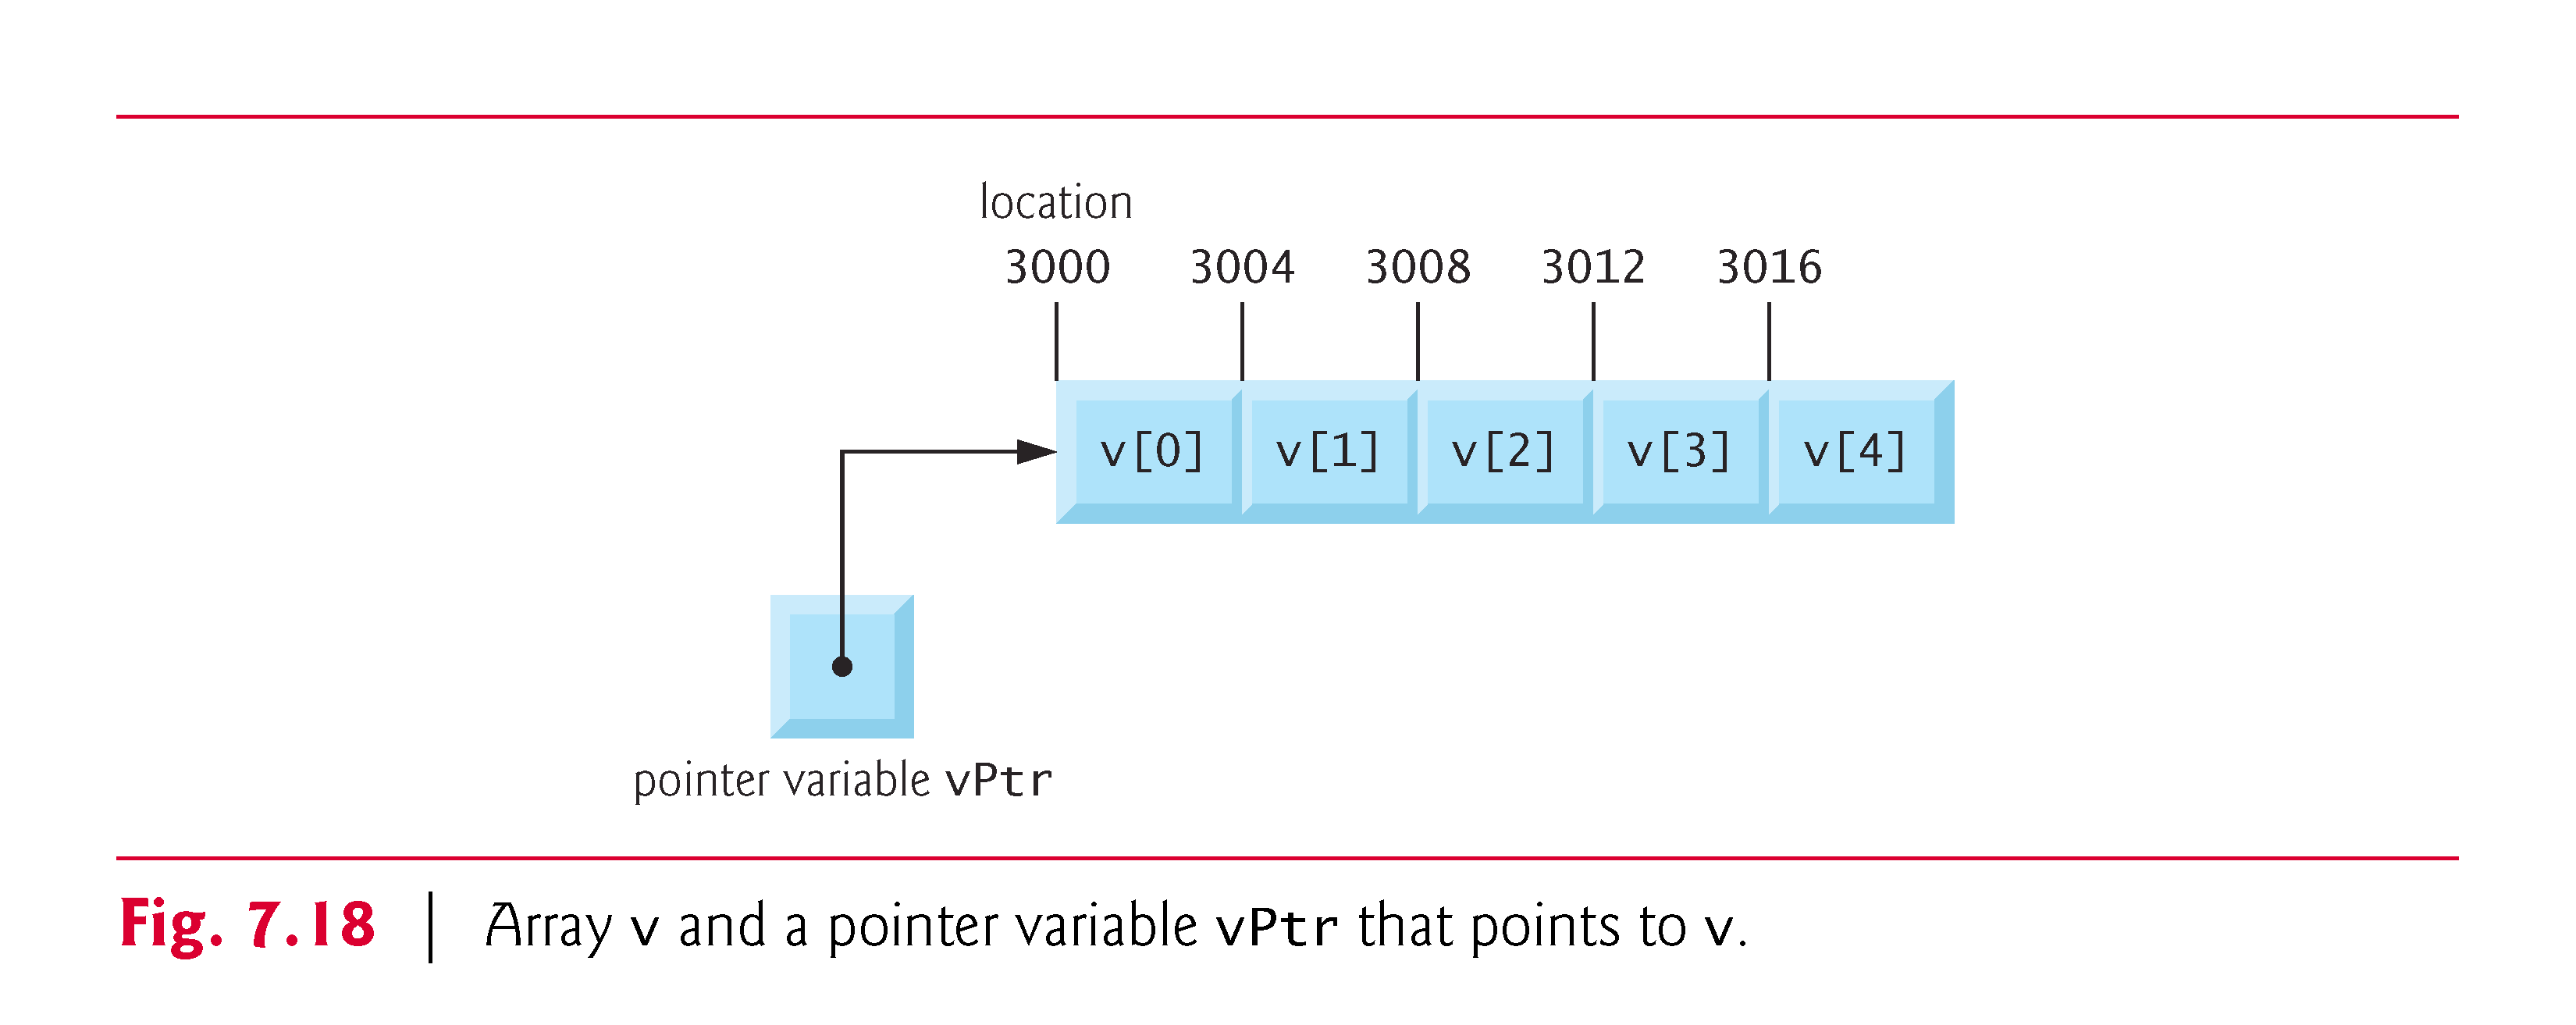
\includegraphics[scale=0.1]{tbe.png}
\end{frame}

\begin{frame}{Our Old Friend \texttt{++}}
\begin{itemize}
\item Notice in the previous slide how \texttt{foo}'s memory addresses are 4 bytes apart, and \texttt{bar}'s are 2 bytes apart.
\item The array is continuous memory, and each element is allocated the size of the base data type of the array.
\item If we wish to perform pointer arithmetic to traverse an array, the compiler needs to how big the steps are!
\end{itemize}
Operators can mean different things when applied to arguments of different types.
\begin{itemize}
\item Float vs Int division, for example.
\item \texttt{++}, when applied to a pointer, will automatically take the size of the data type its operating on! 
\end{itemize}
\end{frame}

\begin{frame}[fragile=singleslide]{Traversing an Array with Pointer Arithmetic}
\begin{lstlisting}[style=C]
#include<stdio.h>
int main(void){
	char foo[] = "Dated Reference";
	char *fooPtr = foo;
	while (*fooPtr != '\0') {
		printf("(%c)", *fooPtr++);
	} 
	printf("\n");
}
\end{lstlisting}
Output:
\hrule
\begin{verbatim}
(D)(a)(t)(e)(d)( )(R)(e)(f)(e)(r)(e)(n)(c)(e)
\end{verbatim}
\end{frame}

\begin{frame}{Other Pointer Operations}
The following are valid operations on pointers:
\begin{itemize}
\item \texttt{++}, \texttt{--}, \texttt{+}, \texttt{-}, \texttt{+=}, \texttt{-=}
\end{itemize}
In each of these cases, the number you are adding/subtracting to/from the pointer is \emph{implicitly multiplied by the byte-width of the data type}.
\begin{itemize}
\item For example, if \texttt{ptr} points to an \texttt{int}, then \texttt{ptr += 4} would move the pointer by 16 bytes, since the bit-width of an \texttt{int} is 4 bytes.
\end{itemize}
Pointers may also be subtracted from one another, but only meaningfully if they point to the same array.
\begin{itemize}
\item \texttt{ptrA - ptrB} yields the number of \emph{array elements} difference between the two pointers, \emph{not} the number of bytes difference.
\end{itemize}
\end{frame}

\begin{frame}{A Word to the Wise...}
\begin{itemize}
\item In the previous example tracing a character array, we used our knowledge that strings are null terminated to set a stopping condition for our loop.
\item Pointer arithmetic can easily place a pointer outside the bounds of its original data structure.
\item There is no in-built protection against out-of-bounds pointers, so we can easily use them to assign to memory outside the array bounds.
\item This could overwrite other variables, cause segmentation faults, and many other troubles! 
\item Back in the day, this was a common exploit used to \emph{hack the government!}. 
\end{itemize}
\end{frame}

\begin{frame}[fragile=singleslide]{Wildcard Pointers}
Normally, pointers require compatible types to be assigned to each other.
\begin{itemize}
\item The exception to this is a \textbf{void pointer}
\end{itemize}
\begin{lstlisting}[style=C]
void *wildcard;
\end{lstlisting}
\begin{itemize}
\item This is a generic pointer that can point to any data type.
\item A void pointer is compatible with all data types, and may be used in assignment operations freely
\item The catch is a void pointer may not be dereferenced.  
\item This is because the dereferencing operation uses the byte width of the pointer's data type to select the area of memory to return. 
\end{itemize}
\end{frame}

\begin{frame}{Operator Miscellany}
Equality and relational operators work on pointers! 
\begin{itemize}
\item Relation operators are only meaningful if the pointers refer to the same data structure! 
\item Equality comparison with \texttt{NULL} is common.
\end{itemize}
Array indexing is actually syntactic sugar for pointer arithmetic! 
\begin{itemize}
\item \texttt{foo[3]} $\equiv$ \texttt{*(foo + 3)}
\item Therefore, it is also possible to index pointers in the same way as arrays! 
\item One of the few differences between pointers and array identifiers is that a array identifiers may not be assigned to.  
\begin{itemize}
\item We can think of them as \emph{read only pointers}.
\end{itemize}
\end{itemize}
\end{frame}

\section[malloc]{Dynamic Memory Allocation}
\begin{frame}{Dynamic Memory Allocation!}
Up to now, our array sizes have been hard-coded (that is, set in the program code itself, not at runtime).
\begin{itemize}
\item In this section, we will learn how to allocate memory dynamically, allowing us to expand or contract arrays as needed at runtime. 
\begin{itemize}
\item When we use static arrays, these memory operations are \emph{implicit}.
\item The general proceedure is to declare a pointer, invoke a memory allocation operation, and store the resultant memory address in the declared pointer.
\end{itemize}
\end{itemize}
We will learn about the following functions, contained in \texttt{stdlib.h}
\vspace{-1em}
\begin{itemize}
\item \texttt{malloc()}
\item \texttt{free()}
\item \texttt{calloc()}
\item \texttt{realloc()}
\end{itemize}

\end{frame}

\begin{frame}[fragile=singleslide]{\texttt{malloc()} - Memory Allocation}
Dynamic allocation of a single, large block of memory, given a specified size.
\begin{lstlisting}[style=C]
int *ptr = (int*) malloc(100*sizeof(int));
\end{lstlisting}
\begin{itemize}
\item \texttt{malloc()} accepts as an argument the number of bytes to allocate, expressed as an integer.
\item It produces a void pointer, which may be type-cast to the type of the pointer you wish to store the address in.  
\item \texttt{malloc()} may fail, if the requested memory is larger than the available memory.
\begin{itemize}
\item In this case, a \texttt{NULL} pointer will be returned.
\item You should always check a pointer returned from \texttt{malloc()} for null status before using it.
\end{itemize}
\end{itemize}
\end{frame}

\begin{frame}{\texttt{malloc()} Broken Down}
\center
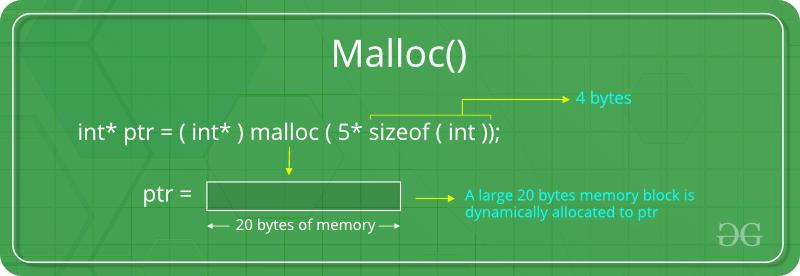
\includegraphics[scale=0.4]{Malloc-function-in-c.png}
\end{frame}

\begin{frame}{No \texttt{free()} Lunches}
We now know how to allocate memory, so let's talk about how to deallocate memory.
\begin{itemize}
\item Memory manually allocated using \texttt{malloc()} \emph{must} be deallocated manually as well.
\begin{itemize}
	\item To \textbf{deallocate} is to take memory allocated to a program, and return control of that memory to the operating system.  
	\item If no program deallocated the memory it used, you would have to restart your computer \emph{very frequently!}
\end{itemize}
\item The \texttt{free()} function accepts a pointer as an argument, and deallocates the memory pointed to.
\item While it is not enforced by the compiler, freeing dynamic memory is the same as closing filestreams: Very good practice.  
\end{itemize}
\end{frame}

\begin{frame}{No \texttt{free()} Lunches (cont.)}
\center
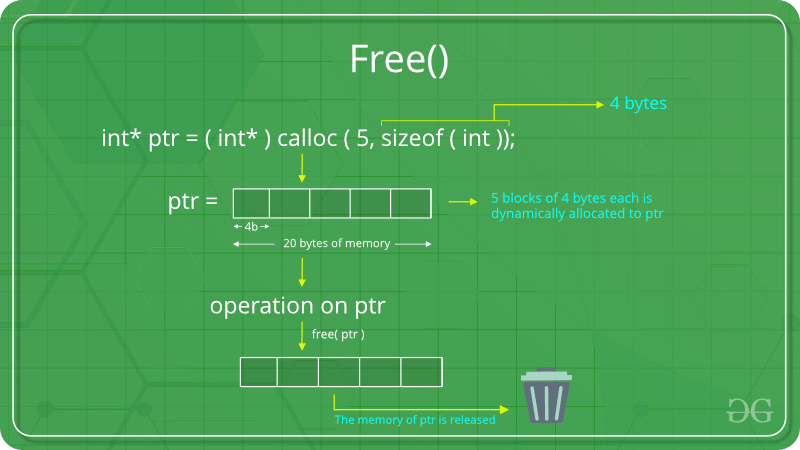
\includegraphics[scale=0.35]{Free-function-in-c.png}
\end{frame}

\begin{frame}[fragile=singleslide]{An example using \texttt{malloc()} and \texttt{free()}}
\begin{lstlisting}[style = C]
void mallocDemo (int n) {
	int* ptr = malloc(n*sizeof(int));
	if (ptr == NULL) {
		printf("Runtime Error!"); 
		return; 
	}
	printf("The memory location allocated is %p\n", ptr);
	for (int i = 0; i < n ; i ++) { 
		ptr[i] = i; 
	}
	printf("The allocated array is : ");
	printArray(ptr, n);
	free(ptr); return;
}
\end{lstlisting}
\end{frame}

\begin{frame}[fragile=singleslide]{\texttt{calloc()} : Memory Allocation For the Hygiene Obsessed}
An alternative to \texttt{malloc()} is \texttt{calloc()}
\begin{itemize}
\item \texttt{calloc()} accepts two arguments:
\begin{itemize}
\item The first is the number of chunks of contiguous memory to allocate
\item The second is the size of these chunks of memory in bytes.  
\end{itemize}
\item Additionally, \texttt{calloc()} wipes all allocated memory (i.e., writes 0 to each chunk).
\item Aside from this, usage is exactly the same as \texttt{malloc()}.
\begin{lstlisting}[style = C]
int n = 100;
int *ptr = calloc(n, sizeof(float));
\end{lstlisting}
\item \texttt{calloc()} is slower than \texttt{malloc()}, however, as overwriting the allocated memory takes time.  
\end{itemize}
\end{frame}

\begin{frame}{\texttt{calloc()} : Memory Allocation For the Hygiene Obsessed}
\center
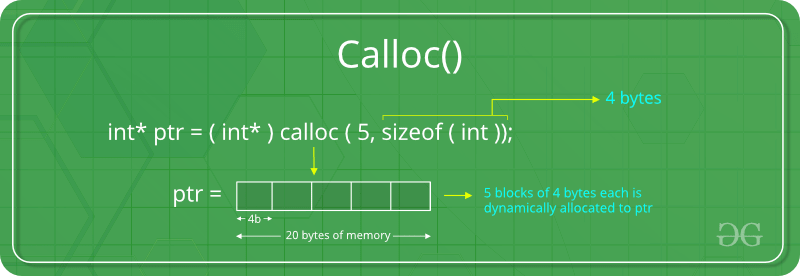
\includegraphics[scale=0.35]{calloc-function-in-c.png}
\end{frame}

\begin{frame}[fragile=singleslide]{\texttt{realloc()} : Change It! Because I Said So!}
So what if we need to dynamically change memory that's been dynamically allocated? 
\begin{itemize}
\item \texttt{realloc()} allows us to change the amount of memory allocated to a pointer, while keeping the data already in it! 
\begin{lstlisting}[style = C]
int *ptr = calloc(40, sizeof(float));
ptr = realloc(ptr, 100*sizeof(float));
\end{lstlisting}
\begin{itemize}
\item The first argument is the pointer to be resized.
\item The second argument is the new size, following \texttt{malloc()} rules.  
\end{itemize}
\item \texttt{realloc()} returns a pointer to the newly allocated memeory
\item New chunks of memory will be filled with smelly garbage! 
\end{itemize}
\end{frame}

\begin{frame}{texttt{realloc()} : Change It! Because I Said So!}
\center
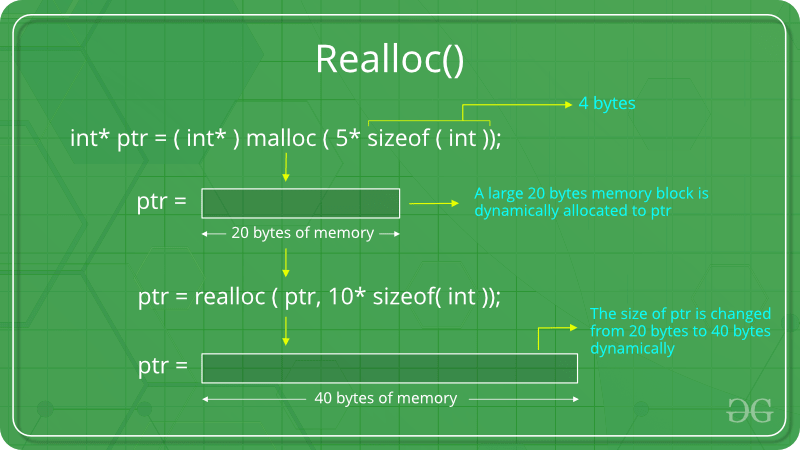
\includegraphics[scale=0.35]{realloc-function-in-c.png}
\end{frame}

\begin{frame}{The Last Slide Comic}
\center
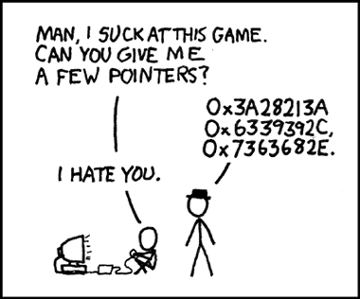
\includegraphics[scale=0.4]{pointers.png}
\end{frame}

\end{document}
